\documentclass[9pt,t,serif,professionalfont,xcolor={table,dvipsnames},noamsthm]{beamer}
\PassOptionsToPackage{pdfpagemode=FullScreen}{hyperref}
\setbeamersize{text margin left = 0.5cm,
               text margin right = 0.3cm}
\mode<presentation>
{
  \usetheme{boxes}
  \setbeamercovered{invisible}
  \setbeamertemplate{navigation symbols}{} 
}
\hypersetup{colorlinks=true,linkcolor=blue} 

\usepackage{../presentation,../presentationfonts}

% load the pdfanim style, should be done after hyperref
% \usepackage{pdfanim}

% load and initialise animation
% arguments:
%   \PDFAnimLoad[options]{name}{xxx}{number}
%   - options: in this example the animation is looped
%   - name: name of the animation
%     (with this name it can be reused several times in the document)
%   - number: number of animation frames / files (n)
% the animation will be composed of files
% xxx0.pdf, xxx1.pdf ... xxx(n-1).pdf


\title{Cardinality}

\author{Jim Hef{}feron}
\institute{
  Mathematics and Statistics\\
  Saint Michael's College\\
  Colchester, VT\\[1ex]
  \texttt{jhefferon@smcvt.edu}
}
\date{}

% This is only inserted into the PDF information catalog.
\subject{Cardinality}

\usepackage{catchfilebetweentags} % read text from background.tex
\newcommand{\catchfilefn}{../../background/background.tex}
% Keep from swallowing end-of-lines
%   https://tex.stackexchange.com/a/40704/121234
\usepackage{etoolbox}
\makeatletter
\patchcmd{\CatchFBT@Fin@l}{\endlinechar\m@ne}{}
  {}{\typeout{Unsuccessful patch!}}
\makeatother

\usepackage{multirow,bigstrut}
\begin{document}
\begin{frame}
  \titlepage
\end{frame}




\section{Cardinality}
% ------------------------------------------------------
\begin{frame}
  \frametitle{Finite sets have the same size iff they correspond}
\ExecuteMetaData[\catchfilefn]{lem:OneToOneOntoFiniteSets}
\begin{center}\small\setlength{\bigstrutjot}{30pt}
  \begin{tabular}{rr|c@{\hspace*{3em}}c}
    \multicolumn{2}{c}{} &\multicolumn{2}{c}{\textit{One-to-one?}}  \\
    \multicolumn{2}{c}{} &\textit{No}  &\textit{Yes}   \\ \cline{3-4}
   \multirow{2}[2]{*}[-8ex]{\it\shortstack{O \\ n \\ t \\ o \\  ?}}
   &\textit{No}
    &\bigstrut\vcenteredhbox{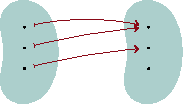
\includegraphics{asy/background02.pdf}} 
    &\vcenteredhbox{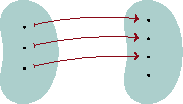
\includegraphics{asy/background01.pdf}}  \\
   &\textit{Yes}
    &\bigstrut\vcenteredhbox{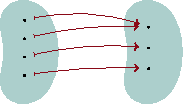
\includegraphics{asy/background00.pdf}} 
    &\vcenteredhbox{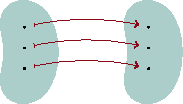
\includegraphics{asy/background03.pdf}}  \\
  \end{tabular}
\end{center}
\end{frame}


\begin{frame}
  \frametitle{Cardinality definition}
\ExecuteMetaData[\catchfilefn]{def:Cardinality}

\pause
\ExecuteMetaData[\catchfilefn]{lem:EquinumerosityIsEquivalence}

\pause
\ExecuteMetaData[\catchfilefn]{def:FiniteInfinite}

\pause
\ExecuteMetaData[\catchfilefn]{def:Countable}
\end{frame}


\end{document}




